\documentclass[../thesis.tex]{subfiles}

\begin{document}

In this chapter, we propose a model-based local planner for high-speed maneuvering in the off-road navigation application. In order to overcome the highly unpredictable vehicle dynamic in the unstructured terrain, we first derive our vehicle model with a data-driven fashion. The high-dimensional vehicle model is used as a standpoint of our model-predictive local planner, which uses Rapidly-exploring Random Tree (RRT) \cite{kuffner2000rrt} as its template. 

Despite the fact that sample-based algorithms are generally more suitable for high-dimensional state space planning, it is not naturally designed for kinodynamic planning to operating in control space. To overcome it, our planner slightly departs from the standard RRT so as to perform at least a certain level of trajectory optimization given the limited computational cycle. The cost function is designed using traveling time in order to encourage the vehicle for a more aggressive maneuvering. 

Several methods are investigated for obstacle detection, with the final version implemented with height map algorithm. A simplified version of occupancy grid is built in global frame when vehicle is moving. Finally, the proposed planner is tested on a full-size all-terrain vehicle (ATV) in the off-road environment. We show that 
Our planner is capable of performing smooth but aggressive high-speed maneuvering, and successfully avoid static obstacles on turnpike with vehicle velocity up to $30 kph$.

The chapter is organized as follows:
Section \ref{sec:vehicle_model} summarizes the derivation of two vehicle models. In Section \ref{sec:rrt-planner}, we introduce our sample-based planner, and detail each specific technique implementation we design. Finally, Section \ref{sec:vehicle_model} shows the experimental results for the vehicle model, and the videos of high-speed navigation on a full-size all-terrain vehicle.

\section{Vehicle Response Model} \label{sec:vehicle_model}

\begin{figure}[t]
	\centering
	\begin{subfigure}[b]{0.18\linewidth}
		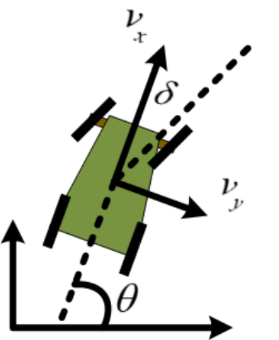
\includegraphics[width=\columnwidth]{./RRTPlanner/fig/vehicle_frame.png}
		\subcaption{}
		\label{fig:vehicle_model_frame}
	\end{subfigure}
	\begin{subfigure}[b]{0.8\linewidth}
		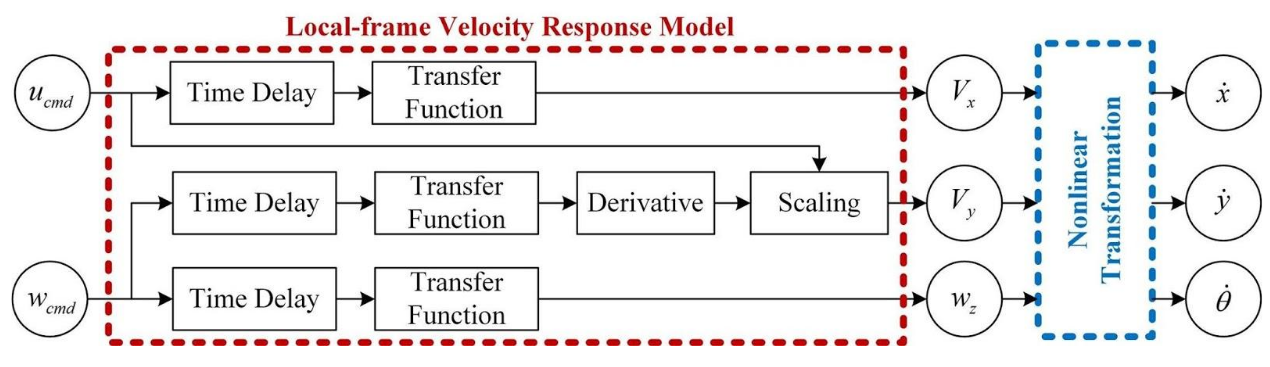
\includegraphics[width=\columnwidth]{./RRTPlanner/fig/vehicle_model_block.png}
		\subcaption{}
		\label{fig:vehicle_model_block}
	\end{subfigure}
	\begin{subfigure}[b]{0.8\linewidth}
		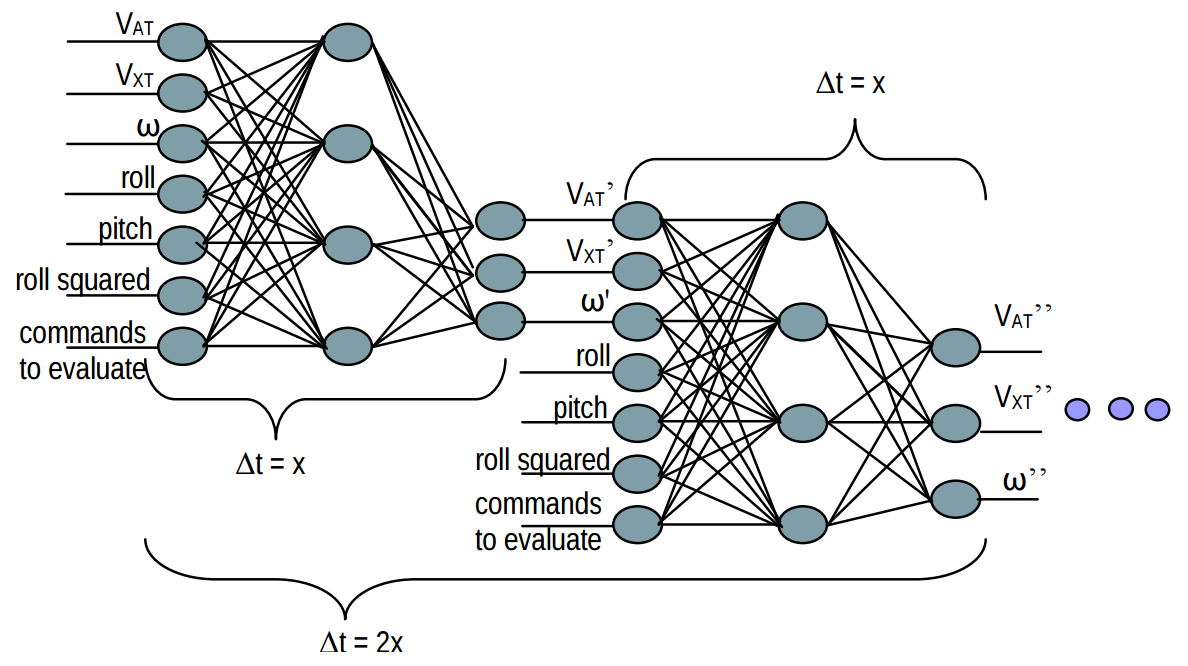
\includegraphics[width=\columnwidth]{./RRTPlanner/fig/neuralnet_model.png}
		\subcaption{}
		\label{fig:vehicle_model_net}
	\end{subfigure}
	\caption{(a) Notation of vehicle velocity in local frame. (b) Data flow of conventional dynamic response model. The model takes two velocity control commands as input and estimates the velocity response in vehicle frame. (c) Schematic illustration of neural-network based response model from \cite{bode2007learning}.}
    \label{fig:vehicle_model}
\end{figure}

% Simulating trajectory 

The forward predictive model $\dot{x}=f(x,u)$ is defined as the function that maps the control action $u \in \mathcal{A}$ and the current state $x \in \mathcal{S}$ into the next state after certain time step $dt$. For unmanned ground vehicle (UGV) in off-road environment, it can be addressed in a modular fashion \cite{kelly2007terrain,howard2006trajectory,howard2005terrain}, where specialized algorithms were developed for each sub-system and later integrated with some fine tunings. Though this modularized approach offers rich semantic representation to allow researchers to better examine the performance of each module, the accumulating errors due to the imperfect approximations propagate to harm the overall performance. 

In fact, modeling sub-systems such as actuator dynamic, vehicle suspension model, and wheel-terrain interaction can be very complex and computational expensive. Here, we limit our scope to a more intuitive yet effective method. Instead, we modeled the predictive model with an unified dynamic model in a more end-to-end fashion. While the control space consists includes forward and rotational velocity, the simulated state is represented as velocity response of vehicle local frame $[v_x, v_y, w]$, as shown in Fig. \ref{fig:vehicle_model_frame}. Once we have the local frame velocity response, we can simply integrate through time to obtain the relative position. 

We derive the model with two different approaches. The first approach based on the standard system identification process, and the corresponding block diagram is shown in Fig. \ref{fig:vehicle_model_block}. It is worth mentioned that the sliding velocity $v_y$ is not negligible on the rough terrain, and in fact plays an crucial role for off-road application. As shown in the blue line in Fig. \ref{fig:velocity_simulate}, the lateral velocity stimulates when the new issued rotational command differs from the previous one, and exponentially decay over time. From this observation, we formulate the lateral velocity response model by using rotational control to stimulate the peak and fine tuning by a scaling ratio proportional to the forward velocity.

%% TODO may consider remove this part, becuz it's a bit lack of technical insight
For the second approach, we implement the neural-network model based on previous work \cite{bode2007learning}. As shown in Fig. \ref{fig:vehicle_model_net}, the neural network takes additional information, such as roll, pitch, and yaw angle, as its input. Note that the squared roll angle is also provided as the fact that from a dynamic standpoint, the vehicle should respond in a near symmetrical manner if it is rolled to the right or rolled to the left. We verified the performance of two models, named as \textit{Conventional Dynamic Model} and \textit{NNet Model}, with our baseline kinematic model on the full-size all-terrain vehicle in Section \ref{sec:rrt-experiments}.


\section{Planner Design} \label{sec:rrt-planner}


\begin{figure}[t]
	\begin{center}
		\centerline{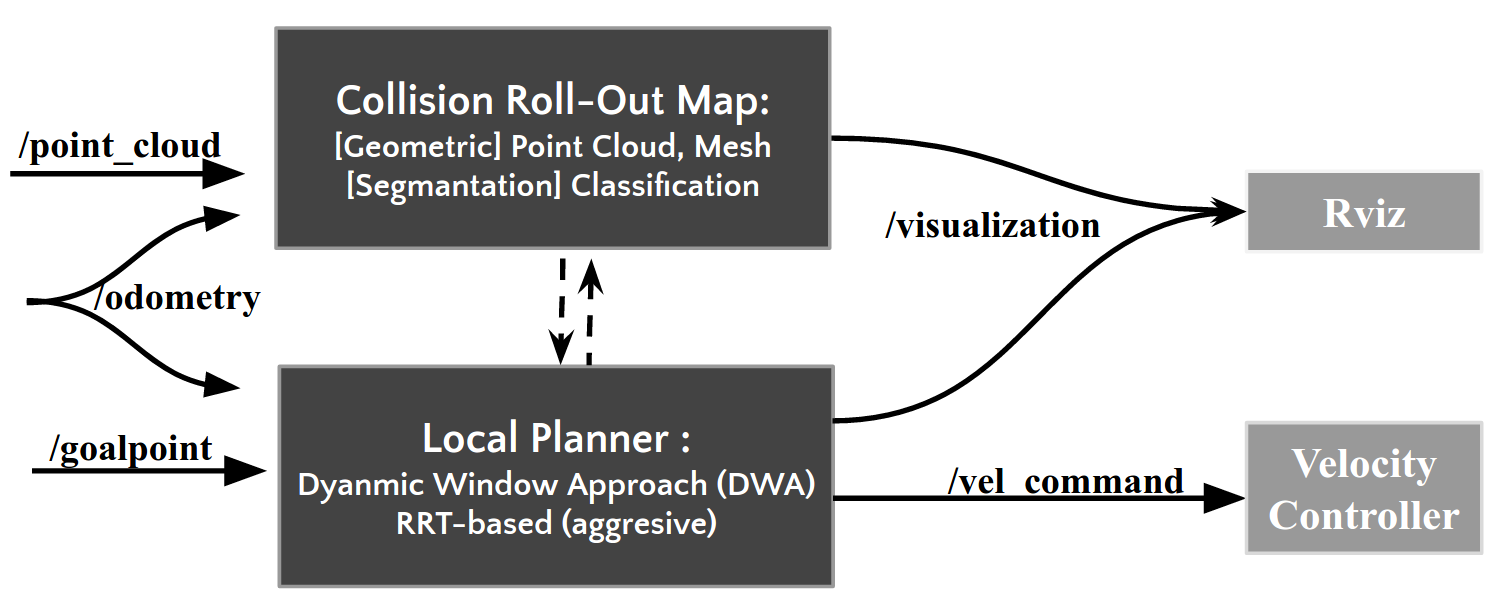
\includegraphics[width=0.8\columnwidth]{./RRTPlanner/fig/planner_module.png}}
		\caption{Block Diagram of our planner API.}
		\label{fig:planner_module}
	\end{center}
\end{figure} 

The block diagram of our planner is shown in Fig. \ref{fig:planner_module}. It can be separated into two modules with respect to functionality. The collision check module constructed a global simplified occupancy grid from vehicle current odometry and pure point cloud data, then communicated with RRT-based planner for collision check service. The velocity command is generated by planner and sent directly to the on-board velocity controller for execution. The detail of two modules is described as follow:


\subsection{Collision Check Module}

Occupancy grid is a commonly-used data structure for obstacles detection. It stores one or multiple probabilities in each grid cell, and increases or decreases them based on sensor model. Since our testing scenario is relatively flat without noise, a simplified version of occupancy grid is used in the matter of fast implementation, in which we replaced the probabilities with a counter. Three different methods for obstacles segmentation were investigated and described below:

\begin{figure}[t]
	\centering
	\begin{subfigure}[b]{0.3\linewidth}
		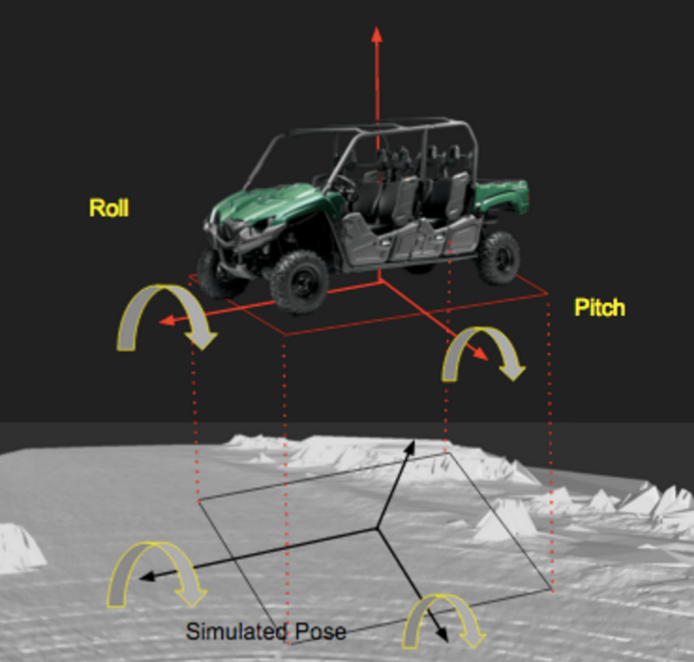
\includegraphics[width=\columnwidth]{./RRTPlanner/fig/mesh.png}
		\subcaption{Mesh with ODE simulation}
		\label{fig:collision_mesh}
	\end{subfigure}
	\begin{subfigure}[b]{0.3\linewidth}
		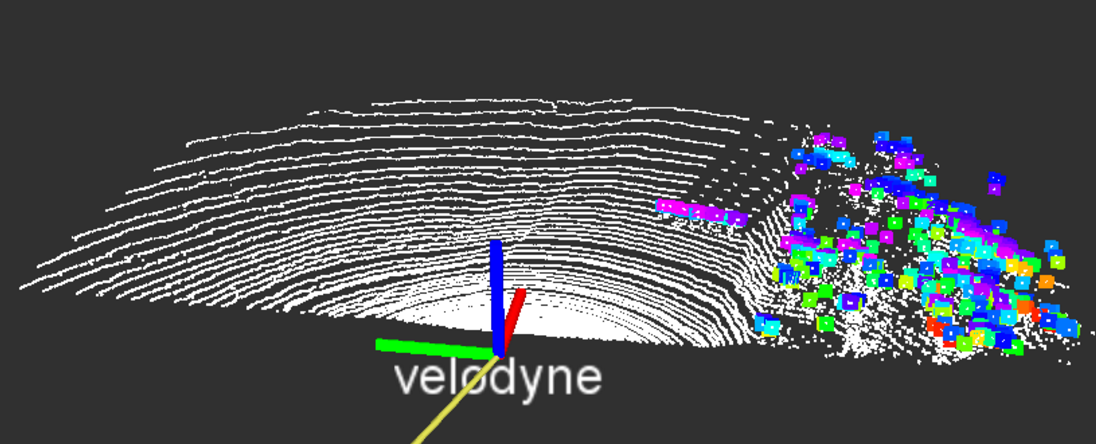
\includegraphics[width=\columnwidth]{./RRTPlanner/fig/ransac.png}
		\subcaption{RANSAC segmentation.}
		\label{fig:collision_ransac}
	\end{subfigure}
	\begin{subfigure}[b]{0.3\linewidth}
		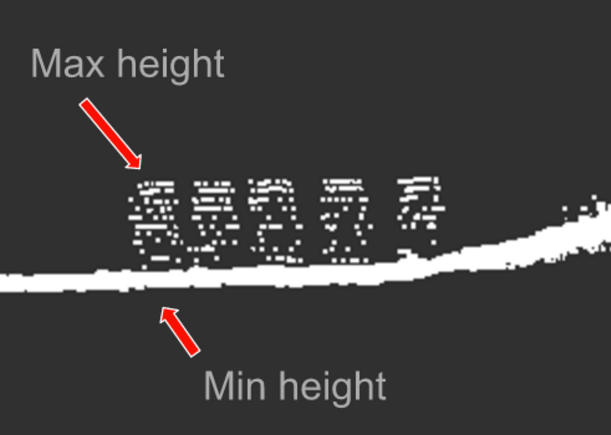
\includegraphics[width=\columnwidth]{./RRTPlanner/fig/height_map.png}
		\subcaption{Height map algorithm}
		\label{fig:collision_height_map}
	\end{subfigure}
	\caption{Three different methods of collision check. Note that for (b), the original and the the processed point cloud is represented with white and colored dot, respectively.}
    \label{fig:collision}
\end{figure}


\subsubsection{i. Mesh Representation with Simulation in Open Dynamic Engine (ODE) \cite{wettergreen2012developing}}
The original method implemented on the vehicle uses ODE and mesh data to simulate the vehicle pose on the ground. Collision is reported if an intersection was detected between vehicle and mesh or the simulated roll and pitch were beyond user-defined thresholds. 

\subsubsection{ii. Plane Removal with RANSAC Segmentation \cite{fischler1981random}}
The second approach for collision check module is using RANSAC segmentation from Point Cloud Library (PCL) to fit the plane model. In our case, the plane model is the ground of our testing environment. We extract the outliers from RANSAC for obstacle detection. As shown in Fig. \ref{fig:collision_ransac}, the white point cloud is the original data, while the colored point cloud is the outliers from RANSAC. 

\subsubsection{iii. Height Map Algorithm}
The third method we used is height map algorithm. This is a simple and efficient algorithm in terms of computation. It calculates the height differences within one grid. If the height difference is greater than user-defined threshold, it will be categorized as an obstacle. As shown in Fig. \ref{fig:collision_height_map}, the artificial obstacle is approximately 1.5 meters. We set the threshold to be 1 meter. Thus it will be recognized as an obstacle. 

% conclusion
Since collision check is the most computationally expensive part of our system and we cannot afford to collide our platform with the obstacles. Efficiency and reliability are the most important requirements. The mesh representation is a good approach for future application such as driving on rough terrain. However, it was not feasible for our scenario in terms of computation consumption. The RANSAC segmentation is sensitive to off-road conditions; the plane model cannot be perfectly fit on rough terrain. In addition, the dusty environment in off-road driving create noises and interference to the Lidar. Considering our requirements and the discussion mentioned above, we choose height map algorithm as our final approach. It’s the fastest and the most reliable. Furthermore, to optimize the computing efficiency, we used bitwise operation instead of multiplication and the obstacle size are dilated to increase robustness of our system. 

\subsection{Sample-based Planner Module}

% Intro
Instead of using traditional search-based planner such as \textbf{A*} or \textbf{D*}, we use a sample-based planner as our development platform. This critical choice comes from an insight that sample-based planner is more efficient for solving a high dimensional planning problem, which gives us a powerful tool when we want to utilize a more complex dynamic vehicle model for state propagation. Besides, maneuvering in wilderness can be seen as a generalized planning problem where discretizing the world based on resolution might not generate a smooth path.

\subsubsection{Simulation}

\begin{figure}[t]
	\centering
	\begin{subfigure}[b]{0.3\linewidth}
		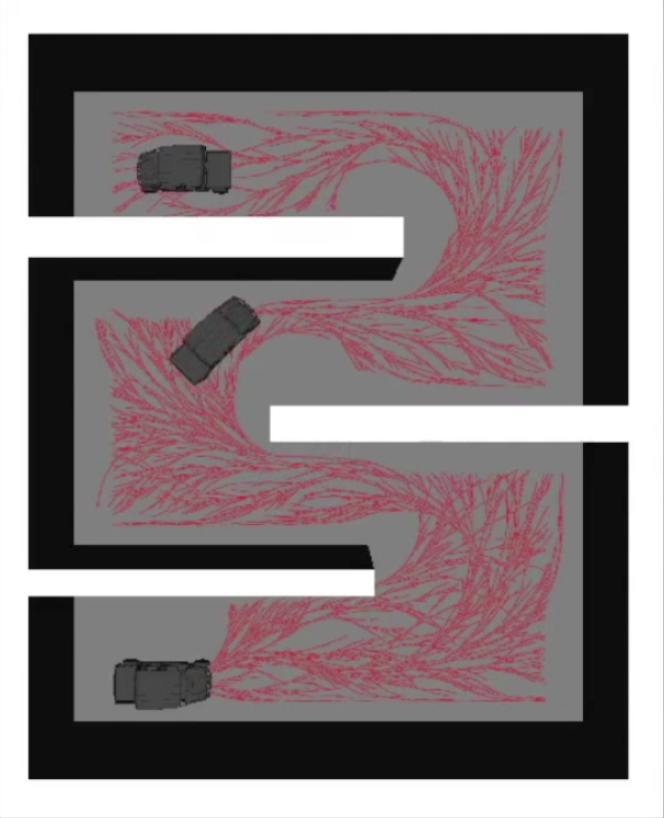
\includegraphics[width=\columnwidth]{./RRTPlanner/fig/rrt-sim-maze1.png}
		\subcaption{}
		\label{fig:rrt-sim-maze1}
	\end{subfigure}
	\begin{subfigure}[b]{0.3\linewidth}
		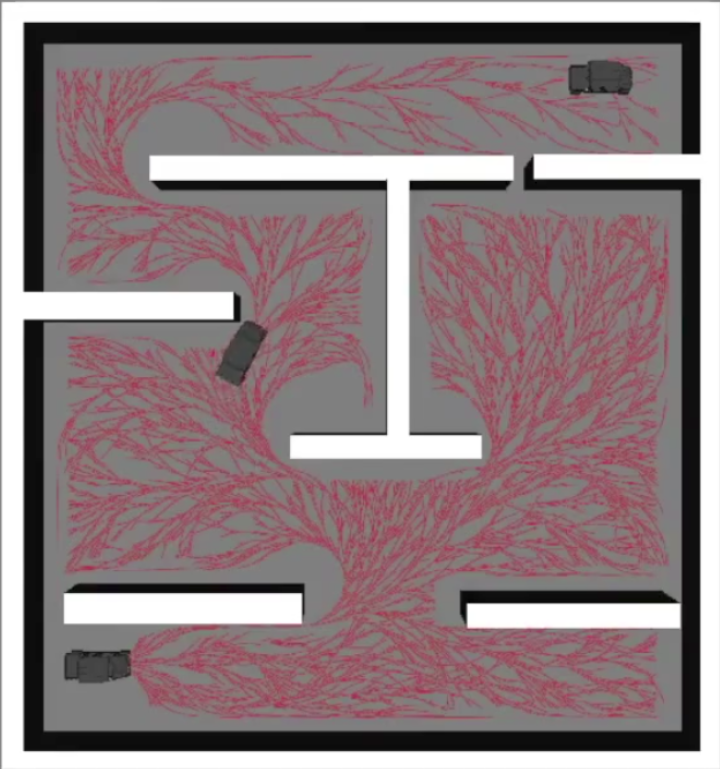
\includegraphics[width=\columnwidth]{./RRTPlanner/fig/rrt-sim-maze2.png}
		\subcaption{}
		\label{fig:rrt-sim-maze2}
	\end{subfigure}
	\caption{Simulation of RRT planner with vehicle model derived in Sec. \ref{sec:vehicle_model}}
    \label{fig:rrt-sim-maze}
\end{figure}


\begin{table}[t]
	\centering
	\caption{Simulation Benchmark}
	\label{table:simulation-benchmark}
	\begin{small}
	\begin{sc}
	\begin{tabular}{ccccc}
		\toprule 
			& PDST \cite{ladd2005motion} & EST \cite{hsu1997path} & RRT \cite{kuffner2000rrt} & KPIECE \cite{csucan2009kinodynamic} \\
		\midrule \midrule
		time & 15.04 & 15.05 & \textbf{15.03} & 15.07 \\
		solution clearance & 1.63 & 1.54 & \textbf{1.38} & 1.70 \\
		solution difference & 1.05 & 1.11 & \textbf{0.98} & 1.30 \\
		\toprule
	\end{tabular}
	\end{sc}
	\end{small}
\end{table}

% Simulation
Our planner is built upon Open Motion Planning Library (OMPL) \cite{sucan2012the-open-motion-planning-library}, an open-source motion planning library that includes a wide range of sample-based planners and a built-in simulation platform \textit{OMPL.app}. We decide our sampled-based planner based on a simple maze navigation simulation using the vehicle response model derived in the previous section. \footnote{Simulation on \textit{OMPL.app}: \url{http://ppt.cc/sBLAh}} The benchmark result is shown in Table \ref{table:simulation-benchmark}, which we observe that the RRT algorithm gives a faster solving time and a smaller path clearance under our vehicle model constraint. With other advantages such as flexibility, we use RRT as our planner template and extend it tor our own purpose. (Fig. \ref{fig:rrt-sim-maze})


\subsubsection{Implementation Details}

\begin{figure}[t]
	\begin{center}
		\centerline{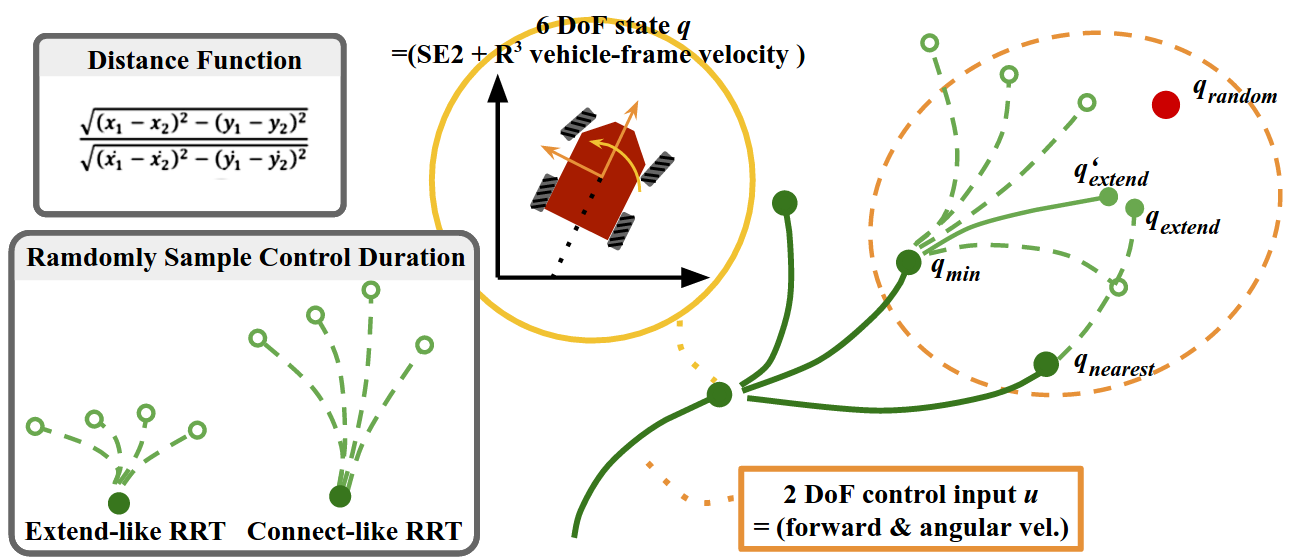
\includegraphics[width=0.8\columnwidth]{./RRTPlanner/fig/rrt.png}}
		\caption{The visualization of RRT-based planner.}
		\label{fig:rrt}
	\end{center}
\end{figure} 

% RRT visualize 
Fig \ref{fig:rrt} visualizes the RRT tree. Each node represents a $6$ DoF states, $q=[x,y, \theta ,v_{forward}, v_{sliding}, w]^T$. The first three terms of the state represent a standard SE2 state space, while the last three terms stand as a vehicle-frame velocity in 2D plane. For control space, we utilize velocity control input, i.e. 2 DoF including forward and angular velocity, since it is commonly-used for autonomous ground vehicle. 
% shooting method and control consistency
During the standard process when RRT extend its leaf, a sequence of control input and its operation duration should be determined in order to propagate toward an extended state $q_{extend}$ after a random state $q_{random}$ is sampled. In order to perform a smooth control throughout the trajectory for off-road navigation, we first uniformly sampled the forward velocity command within an adjustable region. This command region is determined at each iteration based on previously issued command, current vehicle status, and previous executed path such that the vehicle will hold the velocity consistency without jerky output. Then, the shooting method is used to determined the angular velocity command.
% random step size
The standard RRT-like algorithm preserves a fixed extended step size, as shown as the dotted circle in Fig. \ref{fig:rrt}, throughout planning time. While using a larger step size may results in a much smaller solving time yet a jerky trajectory, the trajectory propagated with a smaller step size is usually smoother but computational expensive. The former one is usually referred to \textit{Connected RRT}, and the latter one is called \textit{Extended RRT}. In our implementation, instead of fixing the control duration as a hyperparameter, we randomize the control duration (see ). Our motivations come from the results of our maze simulation, where we observe that tuning the control duration affects the performance of the planner a lot in each different maze configuration. We believe loosening the constraint with such randomly sample mechanism will generalize our planner for various problems. 

% optimization 
Finding an optimal plan is crucial for motion planning but computationally expensive if using a sample -based control-space planner. To overcome it, we implemented a time-optimal RRT* work from Frazzoli \cite{hwan2011anytime}. Moving from RRT toward RRT* includes two more optimization steps in each iteration: (1) reconnecting of extended state, and (2) tree edges trimming. Here, only the first of two optimization steps was implemented because the trimming process in the second step includes updating the whole children tree, which will trade off with planning time. Note that we implemented (1) slightly departs from the standard procedure. Instead of connecting $q_{extend}$ directly to $q_{min}$, we apply shooting method and replace $q_{extend}$ with $q^{''}_{extend}$. The intuition is that in control planning space, it is impossible to propagate to the \textit{same} state in 6 DoF state space. The replace of $q_{extend}$ is accepted only if the new state $q^{''}_{extend}$ is close enough to $q_{extend}$. Finally, We also follow the same setting by using the traveling time instead of standard Euclidean distance in 2D state space as the cost function. The planner thus aims to minimize the traveling time and is encouraged for an agile maneuvering.

% re-planning
The re-planning process is designed as follow: at the beginning of each planner loop, vehicle status, collision check map, and goal point are updated to formulate a RRT control-space planning problem. The problem is solved multiple times, and each of the best solution in each iteration is stored, When the computational time exceeds, the best, i.e. with minimal cost, solution is outputted for execution. Note that the growth tree is abandoned when the next solving iteration starts. In practical we observe such design prevents the planner from publishing poor solution if bad tree structure was built at the beginning of growing stage. We admitted that if an optimal solution can be obtained from one single shot, the replanning setting would have changed significantly \cite{ferguson2006replanning}. Finally, since there is a time delay between the time when vehicle status is updated and the time when the velocity command generated by RRT-based planner is executed, we utilize the same data-driven dynamic model to estimate the vehicle state after such time delay. The parameters used in our local planner are listed in Table \ref{table:rrt-parameters}. 

\begin{table}[t]
	\centering
	\caption{Planner Hyper-parameter}
	\label{table:rrt-parameters}
	\begin{small}
	\begin{sc}
	\begin{tabular}{ccc}
		\midrule \midrule
		\multicolumn{2}{c}{Goal Bias} & 0.7 \\
		\multicolumn{2}{c}{Planner Rate} & 2 Hz \\
		\multicolumn{2}{c}{Solving Rate} & 20 Hz \\
		\multicolumn{2}{c}{Control Duration} & 1.5--6 sec \\
		\multirow{2}{*}{Control Input} & Forward & 10--30 kph \\
		 								& Angular & -0.5--0.5 rad/s \\ 
		\toprule
	\end{tabular}
	\end{sc}
	\end{small}
\end{table}


\section{Experiments and Analysis} \label{sec:rrt-experiments}


\begin{figure}[t]
	\begin{center}
		\centerline{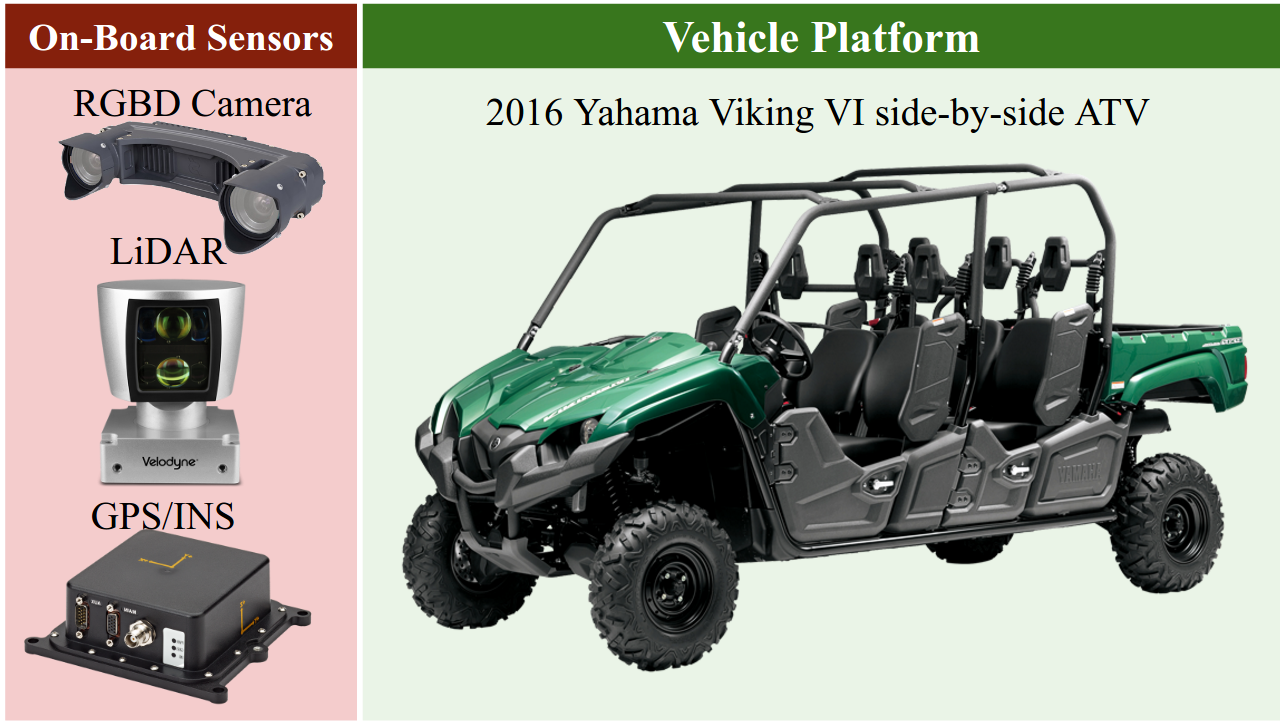
\includegraphics[width=0.7\columnwidth]{./RRTPlanner/fig/viking.png}}
		\caption{The testing vehicle platform and the on-board sensor.}
		\label{fig:viking}
	\end{center}
\end{figure} 

We use Yamaha Viking VI side-by-side ATV as our main testing platform. As shown in Fig. \ref{fig:viking}, the vehicle is equipped with custom drive-by-wire system, velocity controller, and navigation sensors such as GPS/INS, LiDAR, and RGB-D camera. 


\subsection{Vehicle Model Verification}

\begin{figure}[t]
	\begin{center}
		\centerline{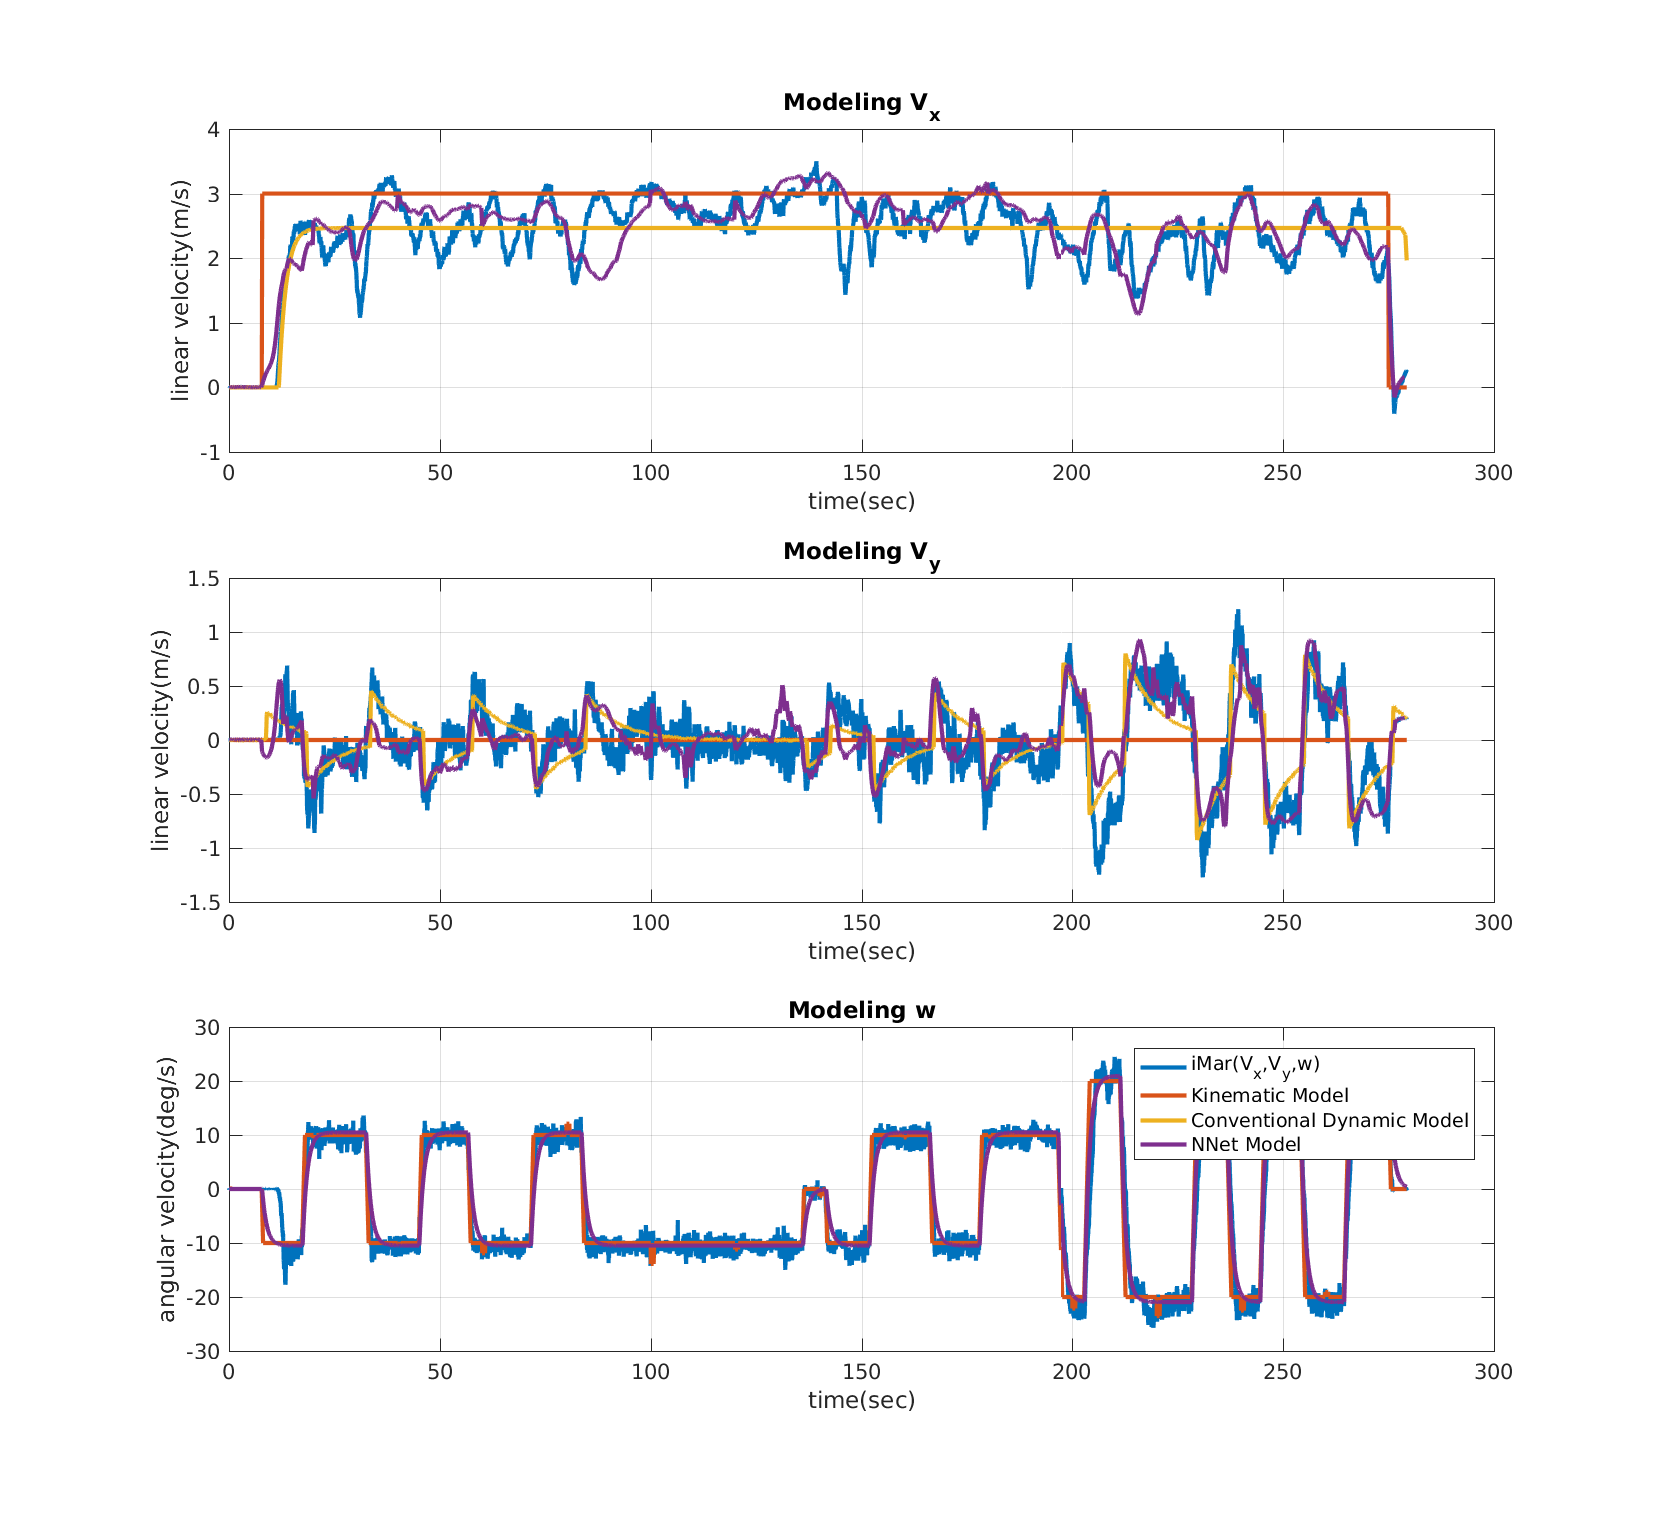
\includegraphics[width=0.8\columnwidth]{./RRTPlanner/fig/simulate_vxvyw}}
		\caption{Simulated velocity response w.r.t. time steps. Note that the blue line is measured under an accurate GPS/INS sensor with RTK signal. We refer this measurement as our ground true data.}
		\label{fig:velocity_simulate}
	\end{center}
\end{figure} 

\begin{figure}[t]
	\begin{center}
		\centerline{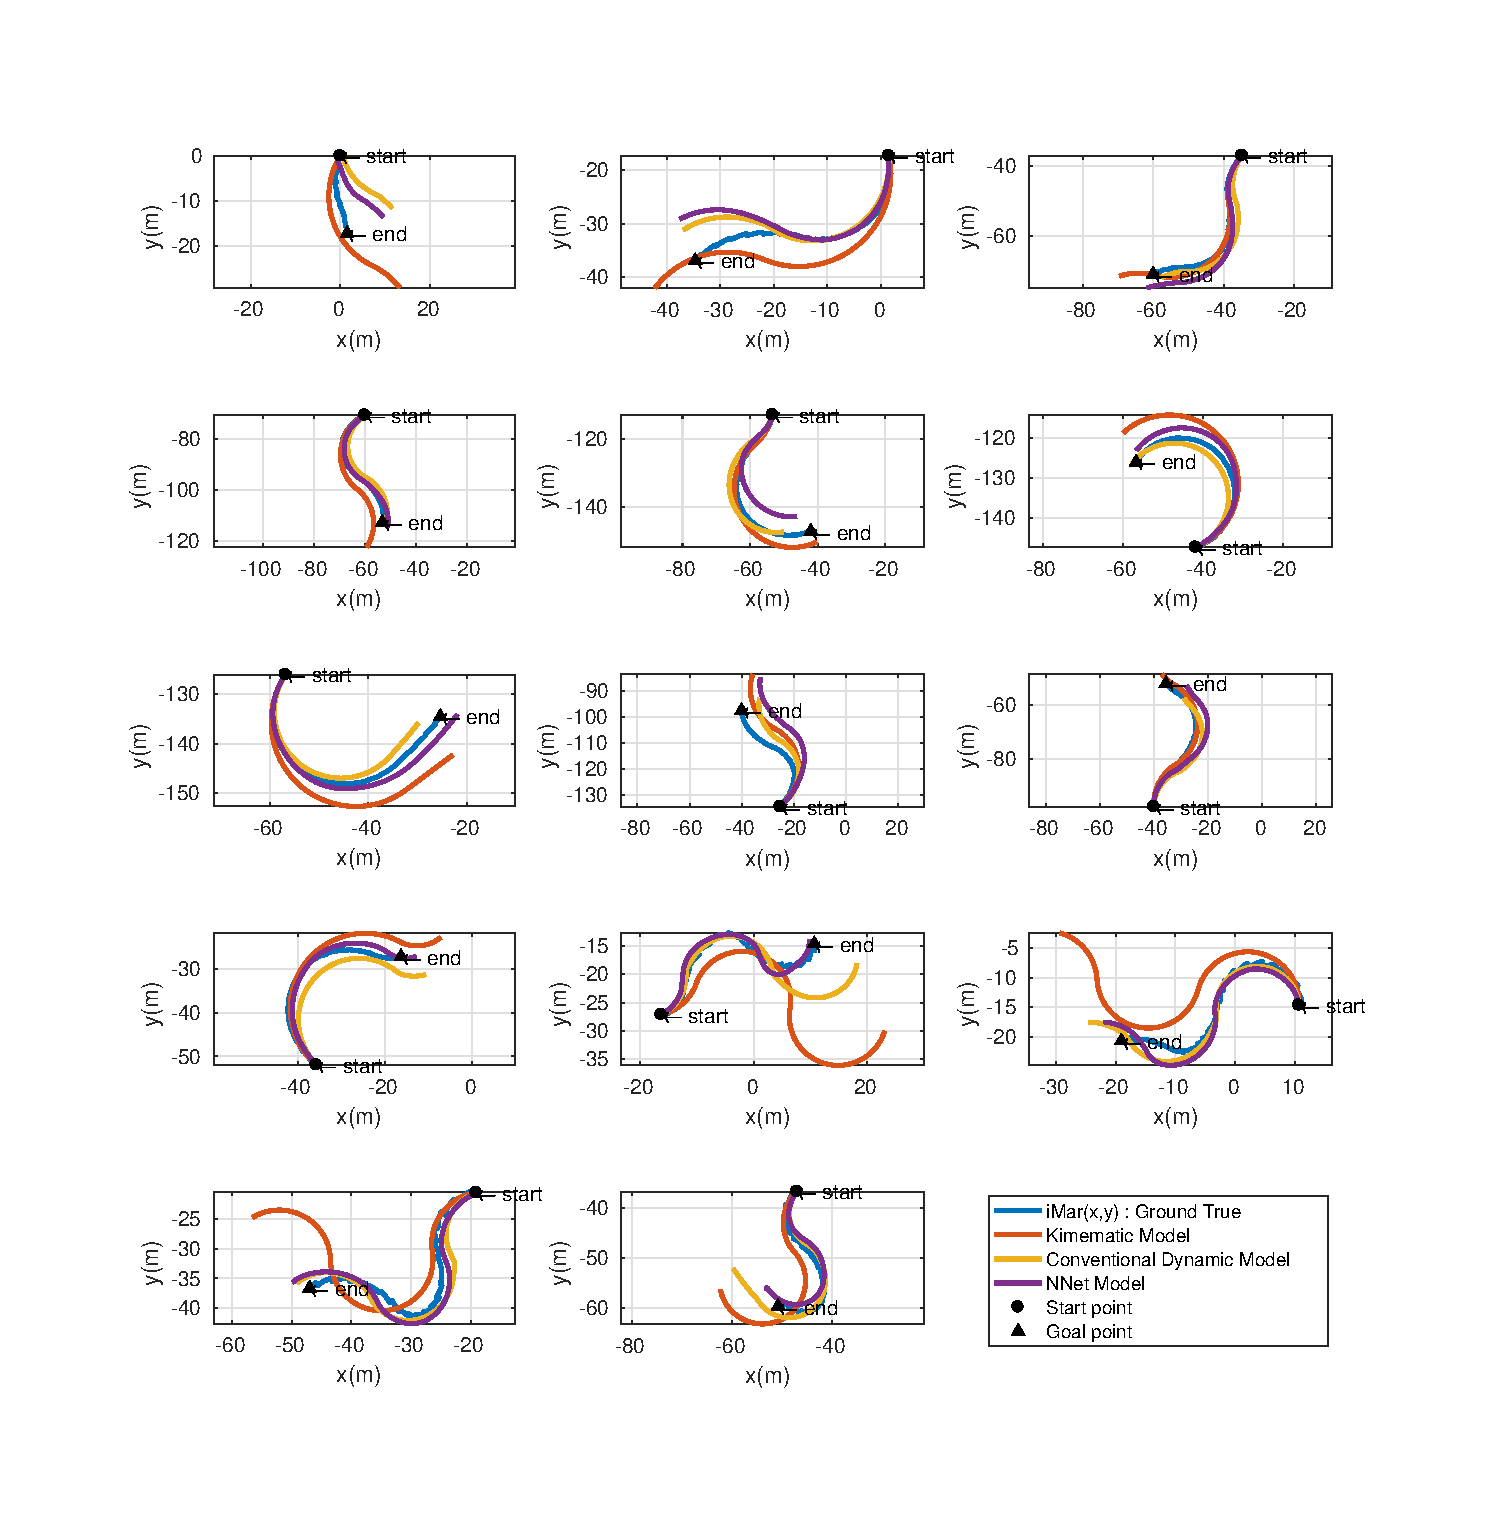
\includegraphics[width=0.8\columnwidth,trim= 0 50 0 160, clip=true]{./RRTPlanner/fig/path_generation_w_nn}}
		\caption{Comparison between data-driven dynamic model and original kinematic model. Note the time interval in each graph is 20 seconds.}
		\label{fig:path_generation}
	\end{center}
\end{figure} 

%% 
The simulated velocity is shown in Fig. \ref{fig:velocity_simulate}, while the integrated relative position is shown in Fig. \ref{fig:path_generation}. The difference from the blue and red line reflects the complex of vehicle model on unstructured terrain. Integrating directly from control command through time, as shown in the blue line, will give a poor result on state propagation. Both of the proposed models are capable to estimate the lateral velocity, which could plays a non-negligible role in off-road cases. However, the conventional dynamic model is not capable to capture the nuance variation of the forward velocity. The neural net model on the other hand gives a better estimation.


\subsection{Planner Demo}

\begin{figure}[t]
	\begin{center}
		\centerline{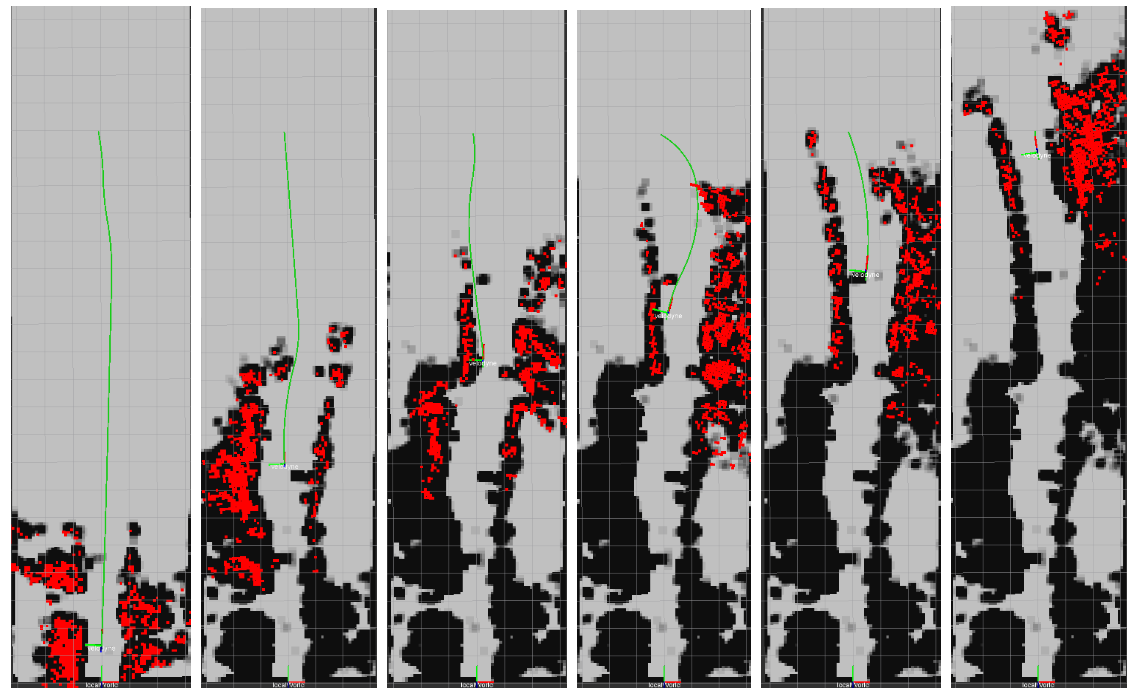
\includegraphics[width=0.8\columnwidth]{./RRTPlanner/fig/demo.png}}
		\caption{Screenshots of planner visualization output. The green path is the trajectory where each point is encoded with a 6 DoF state, 2 DoF control input, and a control duration. The red points are the filtered point cloud segmented as obstacles.}
		\label{fig:demo}
	\end{center}
\end{figure} 

We test our planner on an off-road test field located near Gascola, Penn Hills, PA. 
Our testing scenario is designed as followed: the vehicle should autonomously navigate through a straight turnpike where multiple of static obstacles placed alternatively on both side of track. The static obstacles is 3-meter-length and 1.5-meter height, while the turnpike is a rectangle-shaped field with 10-meter width and 150-meter length. The fastest way to go through the obstacles without any collisions is to perform S-shape maneuvering. Since the standard operating speed ranges from $10$ to $40 kph$, we set the baseline testing speed as $20 kph$ with the top speed of $30 kph$.

In our demo video \footnote{On-field testing with path visualization: \url{https://youtu.be/LibnO8_Sjm0}}, the vehicle successfully avoided all the obstacles at $25 kph$. However, driving at higher speed ($\sim 30kph$) sometimes made collision map vulnerable to noise such as dust and sand blow up when the vehicle drove through, which highly affect the path quality outputted by planner. The example of planning path generation is visualized in Fig. \ref{fig:demo}.

 
% Future works include constructing a more complex model in 3D space, strengthening the collision map with more informative data such as mesh, or classification segmentation, and planner optimization. 

% \section{Discussion}

% \subsection{Traversibility Analysis using DIRL}

\end{document}